\documentclass{subfiles}

\begin{document}

  \chapter{Sistema básico}
  \label{chap:2}

        \section{Estructura}
        \label{sec:2.1}
        Debido a la clara repartición de tareas en cada sección del código, se ha pretendido aplicar una separación tipo Modelo-Vista-Controlador en la aplicación, de manera que todo esté visiblemente separado y se pueda utilizar un sistema de orientación a objetos en toda la parte escrita en \js.

        \paragraph{}
        La primera sección a comentar sería el Modelo. En esta aplicación, tal y como se ha planteado el desarrollo y teniendo en cuenta qué librerías externas se han incorporado y cómo se han utilizado, se ha tratado a estas como si fueran el propio Modelo. Así, nuestra información es en sí las librerías externas añadidas, que serán además las que se encarguen de cargar los datos estáticos de servidor: los modelos en 3D y las grabaciones de las voces de estos.

        \paragraph{}
        La segunda sección sería la Vista. En este caso, la Vista de esta aplicación constaría únicamente de un HTML llamado \textit{index}, que sería además la \textit{landing page} de la aplicación. Sobre esta misma página será sobre la que se colocará más tarde un \textit{<<canvas>>}, que es el elemento HTML que permite mostrar elementos gráficos de manera dinámica a través de \js. Utilizando este último podremos mostrar las imágenes captadas a través de la cámara del dispositivo móvil y mezclarlas con los modelos en 3D para generar nuestra \ra.

        \paragraph{}
        Por último, la sección restante sería el Controlador. En este, se procesan todos los eventos generados por el usuario, además de tratar toda la información que se recibirá de los sensores del dispositivo para poder generar las imágenes de manera verosímil. En este se ubicará un bucle que se ocupará de obtener la imagen a mostrar, mezclarla con el modelo en 3D, renderizar la imagen y situarla en la vista, todo esto de la manera más fluida posible para que el espectador no tenga impresiones que entorpezcan la experiencia de usuario.

        \paragraph{}
        Además, esta almacenará también información de la Sesión necesaria para el correcto procesamiento del sistema, tales como los modelos en 3D cargados, la referencia al objeto de \js con el \textit{<<canvas>>} antes mencionado, la posición del usuario y otros datos necesarios para el funcionamiento del sistema que serán mencionados a lo largo de esta memoria.

        \paragraph{}
        Es importante mencionar que, a pesar de que se ha tratado a este sistema como un Modelo-Vista-Controlador y se le ha presentado como tal, sería más justo tratar a la aplicación como si utilizara el patrón Modelo-Vista-Presentador \cite{web:mvp} por varias razones.

        \paragraph{}
        La primera es que no tenemos constancia de cómo almacenan estas librerías las pocas referencias que se le entregan a la Vista y, aún manteniendo esta referencia como si lo tratara como la Vista en este tipo de patrones, no parece realizar cambios sobre esta de manera directa.

        \paragraph{}
        La segunda es que las actualizaciones se realizan directamente desde el Controlador, siendo necesario realizar desde este último acciones explícitas para actualizar la apariencia de la vista, como por ejemplo el renderizado de la imagen a mostrar en pantalla.

        \paragraph{}
        Por último y más importante, es necesario que todos los cambios estén revisados en el bucle que se genera en el Controlador, el cual se tratará más adelante. Esto obliga a este último a solicitar información continuamente a las librerías, hacer cálculos y mostrarlos en pantalla, mientras está atento a los eventos de los usuarios.

        \begin{figure}
        \centering
        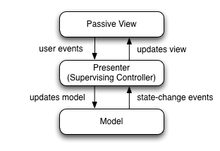
\includegraphics[width=0.5\textwidth]{img/mvp.png}
        \caption{Representación gráfica del patrón Modelo-Vista-Presentador. Imagen obtenida de Wikipedia.}
        \label{fig:mvp}
        \end{figure}

        \paragraph{}
        Por todo esto, y dado que la lógica de negocio está separada de la interfaz de usuario, la estructura se corresponde con el patrón Modelo-Vista-Presentador. Sin embargo, dado que desde el inicio del proyecto se trató cada parte como el clásico Modelo-Vista-Controlador, y dado que el Modelo-Vista-Presentador proviene de este último, cada parte será nombrada como si lo fuera, aún siendo conscientes de las diferencias.

        \section{Sesión WebXR}
        \label{sec:2.2}

        La primera herramienta que será necesario inicializar es una instancia de Sesión de \webxr. La Sesión de \webxr, llamada \textit{XRSession} \cite{web:xrsession}, es el objeto de la librería \webxr que provee de las funcionalidades más básicas, así como de utilidades extra que serán implementadas a lo largo del desarrollo de la aplicación. Esta interfaz pretende representar la propia actividad que llevará a cabo el usuario mientras observa la \ra, por lo que tendrá funciones orientadas a iniciar, mantener y terminar esta actividad.

        \paragraph{}
        Para ser inicializado, el objeto Sesión tiene varios requisitos que se deben cumplir \cite{web:webxrrequirements} para evitar problemas de seguridad. Los dos requisitos mencionados por la documentación de \arcore son:

        \begin{itemize}
            \item {El servidor que ofrezca el servicio debe tener una conexión a través de un entorno seguro. \webxr considerará segura una comunicación que se transmita a través del protocolo \textit{HTTPS} y/o que se ubique en \textit{localhost}}.
            \item {El cliente debe utilizar un navegador compatible con WebXR. A fecha de este documento, solo existen tres navegadores para dispositivos móviles que cumplan este requisito \cite{web:webxrcompatibility}: \googlechrome para \android a partir de la versión 79, \textit{Opera} para \android a partir de la versión 57 y \textit{Samsung Internet} a partir de la versión 11.2. Además, el dispositivo que lo lance debe soportar la aplicación \arcore.}
        \end{itemize}

        Además de esto, la Sesión se debe iniciar a través de lo que el sistema debe interpretar que es un evento de usuario. Esto quiere decir que la Sesión no se puede generar automáticamente o nada más cargarse la página, sino que debe ser el usuario pulsando un botón o realizando una acción consciente el que lance la solicitud de inicio de Sesión de \ra. Los dos primeros requisitos expuestos se comprueban a través de la función \textit{isSessionSupported}:

\begin{lstlisting}[language=JavaScript, caption={Uso de \textit{isSessionSupported en la aplicación}.}, label={lst:2.1}]
if (!navigator.xr) window.polyfill = new WebXRPolyfill();

navigator.xr.isSessionSupported("immersive-ar").then(
    this.#checkSessionSupported
);
\end{lstlisting}

        Esta función (línea 3) está integrada en el parámetro \textit{xr}, que está a su vez contenido en \textit{Navigator}, objeto que contiene información acerca del navegador utilizado por el usuario. Este último contendrá el parámetro mencionado únicamente si cumple con el segundo requisito de la librería \webxr. En caso contrario, al no existir, podría generarse un error. Para estos casos, se utiliza \textit{WebXRPolyfill} \cite{web:webxrpolyfill}, una librería utilizada para la retrocompatibilidad en los navegadores compatibles, pero que también añade el mencionado parámetro y, con este, la funcionalidad que comprueba si se soporta la Sesión.

        \paragraph{}
        La línea 3 del código anterior termina en una llamada asíncrona mediante el uso de \textit{.then()} a la función privada \textit{checkSessionSupported}. Esta función es la que se encarga de avisar al usuario en caso de que la Sesión no se pueda levantar. Sin embargo, en el caso afirmativo, se ocupa de preparar el entorno para el momento en que el usuario comience la sesión de \ra, cuyos detalles se explicarán más adelante.

\begin{lstlisting}[language=JavaScript, caption={Control de la Sesión, dependiendo de si es o no soportada.}, label={lst:2.2}]
#checkSessionSupported = (isSupported) => {
    if (isSupported) {
    
        // Prepara el entorno
    
    } else {
    
        document.getElementById("arButton").disabled = true;
        alert("Tu navegador no permite una sesi\xF3n de Realidad Aumentada.");
        
    }
};
\end{lstlisting}

        Esta estructura de funciones, tan común en \js, es la que se utilizará en este proyecto para las funciones \textit{callback} \cite{web:callbackfunction}, funciones pasadas a otras funciones en forma de argumento de forma que puedan ser llamadas una dentro de la otra. Así, en este caso, la función de la librería calculará si el sistema soporta o no la Sesión y, una vez lo sepa, llamará a nuestra función (\textit{checkSessionSupported}) pasándole como argumento el resultado de sus cálculos.

        \begin{figure}
        \centering
        
\includegraphics[width=0.25\textwidth]{img/landing_page.jpg}
        \caption{Imagen de la \textit{landing page} definitiva de la aplicación web.}
        \label{fig:landing_page}
        \end{figure}

        \paragraph{}
        Teniendo en mente estas condiciones, se planteó que la Vista debía ser una interfaz sencilla que contuviese un botón que debiera accionar el usuario para iniciar la Sesión, siendo en las versiones más prematuras un botón simple sin ningún tipo de customización. En las versiones más avanzadas, se generó un fichero \textit{CSS} que personalizara la \textit{landing page} de manera que, además de tener los colores de la empresa, tuviese un aspecto más amigable para el usuario. Antes de que este botón pudiera ser pulsado, el sistema debería haber calculado previamente si el sistema puede soportar la sesión, así que con la carga de la Vista debía cargarse también el archivo Main.js, que consta únicamente de una línea de código:

\begin{lstlisting}[language=JavaScript, caption={Inicialización del Controlador.}, label={lst:2.3}]
window.arController = new Controller();
\end{lstlisting}

        Esta línea lanzará el Constructor del Controlador, que contendrá la construcción del \textit{WebXRPolyfill} y la consulta al parámetro \textit{xr} con la función \textit{isSessionSupported}. De esta manera, el sistema está previamente preparado a cualquier acción del usuario, favoreciendo la carga de objetos más pesados de manera asíncrona mientras el usuario reacciona antes de pulsar el botón de lanzamiento de Sesión de \ra.

        \paragraph{}
        Ahora, una vez se ha comprobado que el sistema es compatible con \ra, el usuario puede ejecutar su acción consciente para iniciar la Sesión. Es importante tener en cuenta que, cuando se construye el objeto, también puede detectar si la acción es consciente o no, por lo que la construcción de este también debe estar sujeta a un evento de usuario. Debido a esto, la construcción de este objeto no se puede incrustar en el mismo sitio que hemos incrustado la carga de objetos más pesados, junto al lanzamiento de la página, sino que debe ir en la función que se lance al pulsar el botón que se muestra en la Figura \ref{fig:landing_page}.

        \paragraph{}
        Este botón lanzará la función asíncrona \textit{startLoop} (cuyo significado revelaremos más adelante), que cargará los datos restantes para poder ejecutar el grueso de la aplicación, siendo la Sesión uno de ellos, como ya se ha comentado. En esta aplicación, la sesión se lanza de la siguiente manera:

\begin{lstlisting}[language=JavaScript, caption={Función de preparación del bucle.}, label={lst:2.4}]
// Constantes
#GLOPTIONS = { xrCompatible: true };
#SESSIONOPTIONS = { requiredFeatures: ['hit-test'] };
// ...

async startLoop() {
    this.#canvas = document.createElement("canvas");
    document.body.appendChild(this.#canvas);
    this.#gl = this.#canvas.getContext("webgl", this.#GLOPTIONS);

    // ...
    
    this.#session = await navigator.xr.requestSession("immersive-ar", this.#SESSIONOPTIONS);
    this.#session.updateRenderState({
        baseLayer: new XRWebGLLayer(this.#session, this.#gl)
    });

    // ...
}
\end{lstlisting}
        
        En el código se puede observar que, en la línea 13, no se está construyendo un objeto utilizando el constructor clásico \textit{new}, sino que se está solicitando un objeto \textit{XRSession} (Sesión de \webxr) al parámetro \textit{xr} previamente mencionado mediante la función \textit{requestSession} \cite{web:requestsession}. Esta es la manera que tiene \webxr de asegurarse de que la sesión se lanza mediante un evento de usuario, debido a que es precisamente esa función la que recoge la información necesaria y hacer las comprobaciones correspondientes al respecto.

        \paragraph{}
        También se puede observar que la función recibe dos parámetros: la cadena de texto \textit{``immersive-ar"} en primer lugar y \textit{this.\#SESSIONOPTIONS} en el segundo. El primero es un parámetro obligatorio que aclara a la función qué tipo de Sesión se pretende lanzar (\ra, \rv o \textit{inline}, una opción que no nos ocupa ahora), siendo el valor presente en el código el necesario para indicar que queremos solicitar una Sesión de \ra. El segundo valor, opcional en este caso, sirve para especificar la configuración que se establecerá en nuestra sesión, en caso de que no queramos utilizar los valores por defecto. En esta aplicación se establece una única opción, definida en la constante de la línea 2, que indica las características que serán requeridas durante la sesión. En este caso, se indica que será necesaria la característica \textit{hit-test} o, como lo llamaremos para esta aplicación, <<cálculo de superficies>>, aunque eso es algo que explicaremos más adelante.

        \paragraph{}
        Justo después de solicitar la Sesión, se utiliza a esta misma para lanzar la función \textit{updateRenderState} \cite{web:updaterenderstate} en la línea 15. Esta función solicita cambios de configuración a partir del siguiente fotograma que se cargue. Sin embargo, como a estas alturas aún no se ha cargado ningún fotograma, se entiende que estos <<cambios en la configuración>> son para el primero y para los siguientes fotogramas (es decir, para todos, dado que esa configuración no va a cambiar en esta aplicación).

        \paragraph{}
        La configuración que se solicita cambiar para los fotogramas es la que se prepara en las líneas 7, 8 y 9 junto con la constante de la línea 2: en la línea  8, estamos generando un \textit{canvas}, que es un objeto de HTML generado a partir de \js cuya finalidad es albergar objetos gráficos, como ya se mencionó en la sección \ref{sec:2.1}. Para insertar este objeto en nuestra Vista, se ejecuta la acción de la línea 8, momento a partir del cuál este objeto ocupará la pantalla completa de nuestro dispositivo móvil. Si no añadiésemos más funcionalidad, veríamos que nuestra pantalla no mostraría nada más que una pantalla en negro. Esto se debe a que aún no hemos insertado ningún objeto gráfico en nuestro \textit{canvas}, para lo que aún quedan unos pasos.

        \paragraph{}
        Por último, en la línea 9 se solicita al objeto \textit{canvas} un <<contexto>> a través de la función \textit{getContext}. El contexto de un \textit{canvas} es una interfaz a través de la cuál se puede interactuar y generar gráficos e imágenes desde el código de \js \cite{web:canvascontext}, por lo que nos resulta imprescindible para trabajar con este <<lienzo>>. Primero, a la función le indicamos qué tipo de imágenes vamos a utilizar para que nos devuelva el objeto de contexto correcto (en nuestro caso, el contexto va a ser la inserción de imágenes en 3D). Eso lo hacemos mediante el primer parámetro (``\textit{webgl}"), mientras que en el segundo, tal y como ocurrió al solicitar la sesión de \webxr, le establecemos una serie de opciones que queremos que sean distintas a las predeterminadas. En este caso, queremos activar la opción <<\textit{xrCompatible}>>, que indica que indica al \textit{canvas} que el contexto que nos devuelva tiene que ser compatible con \webxr \cite{web:getcontext}. Esta configuración es la que se almacena en la constante de la línea 2.

        \paragraph{}
        Una vez entendido esto, solo queda añadir esta configuración a la función \textit{updateRenderState}. A través del objeto \textit{XRWebGLLayer}, generaremos un objeto que enlace el contexto del \textit{canvas} (es decir, la interfaz para poder dibujar sobre este) y la Sesión \webxr que mantendremos para aplicar nuestra \ra \cite{web:xrwebgllayer}. Esto lo asociaremos con la opción <<\textit{baseLayer}>> a la misma Sesión a partir del momento en que comiencen a lanzarse los fotogramas con la sencilla intención de indicarle a la Sesión cuál será el objeto que le renderizará las imágenes obtenidas desde la cámara del dispositivo. Esto significa que el contexto, a través del enlace creado con el objeto \textit{XRWebGLLayer}, obtendrá la información de la cámara del dispositivo y lo traducirá en la colección de píxeles que plantaremos en el <<lienzo>>.

        \paragraph{}
        De esta manera tendríamos iniciada la forma más básica de Sesión, aunque aún no seríamos capaces de ver nada a través de la pantalla de nuestros dispositivos. Para esto, vamos a necesitar lanzar un bucle en el que procesemos y mostremos los fotogramas que captemos con la cámara de nuestro móvil.
        
        \section{Procesado iterativo}
        \label{sec:2.3}

        Para poder mostrar por pantalla cada fotograma, así como hacer los cálculos relacionados con las figuras que vamos a insertar llegado el momento, es necesario crear un bucle que dure tanto tiempo como el usuario vaya a permanecer en la Sesión. En cada una de las iteraciones, la aplicación solicitará al hardware del dispositivo móvil la imagen captada a través de su cámara.

        \paragraph{}
        Este bucle funcionará de una manera un tanto especial: a diferencia de los bucles \textit{for} o \textit{while}, donde se ejecuta un código de manera secuencial y sin tener nada más en cuenta que lanzar la siguiente iteración cuando la anterior haya terminado, en este bucle se <<solicita>> al navegador que ejecute una función \textit{callback} en cuanto esté preparado, lo que permite que la aplicación se adapte a la capacidad del dispositivo, debido a que no todos serán capaces de procesar igual de rápido la misma información. En esta función \textit{callback}, que definiremos nosotros, será en la que se le indicará al sistema que muestre por pantalla la información que queramos. Esto, a efectos prácticos, es lo que determinará los fotogramas por segundo: si un sistema, desde que se solicita la ejecución de la función hasta que muestra el fotograma en pantalla, tarda 0,025 segundos de media, entonces mostrará en un segundo alrededor de 40 fotogramas (es decir, 40 fotogramas por segundo).

        \paragraph{}
        Esta capacidad para solicitar la ejecución de una función \textit{callback} cuando el sistema esté disponible la tiene la función \textit{requestAnimationFrame} de la Sesión de \webxr \cite{web:requestanimationframe}. Por esto, es imprescindible que la Sesión se haya iniciado previamente. En esta aplicación, la función se lanza en dos puntos dentro del Controlador.

\newpage
\begin{lstlisting}[language=JavaScript, caption={Función que solicita la carga del siguiente fotograma.}, label={lst:2.5}]
async startLoop() {

    // ...
    // Solicitud del primer fotograma
    this.#session.requestAnimationFrame(this.#loopFunction);
    
}
\end{lstlisting}

        La primera llamada a dicha función se realiza al final de la función \textit{startLoop}, que es la función llamada por el botón de la Vista y que, como su propio nombre indica, es la que inicializa este bucle, haciendo ciertas preparaciones antes como el inicio de la Sesión, como ya sabemos. Al lanzar la función \textit{requestAnimationFrame}, es necesario indicarle cuál va a ser la función \textit{callback} que se va a poner <<en cola>> de ejecución. En nuestro caso, esta función es \textit{loopFunction}, donde ejecutaremos nuestro procesamiento de imágenes:

\begin{lstlisting}[language=JavaScript, caption={Función bucle con el contenido mínimo}, label={lst:2.6}]
#loopFunction = (time, frame) => {

    // ...
    // Solicitud de siguiente fotograma
    this.#session.requestAnimationFrame(this.#loopFunction);

    // Enlazado de imagen de camara con modelo
    this.#gl.bindFramebuffer(this.#gl.FRAMEBUFFER, this.#session.renderState.baseLayer.framebuffer);
    // ...
    
};
\end{lstlisting}

        Para poder generar el bucle que se encargará de procesar y mostrar la imagen, es necesario que en algún punto se solicite de nuevo al navegador que se vuelva a lanzar esta misma función. Para ello, el mejor sitio es la propia función \textit{loopFunction}, que solicitará al navegador que se vuelva a lanzar cuando este esté preparado (línea 5), formándose así un bucle infinito, en el que se realizará el procesado que definamos en la función por cada iteración y que terminará cuando el usuario decida, como se explicará más tarde.

        \paragraph{}
        En esta función \textit{callback}, podemos ver que se reciben dos parámetros generados desde la Sesión al llamarla: \textit{time} y \textit{frame} \cite{web:requestanimationframe}. El parámetro \textit{time} es una variable de tipo \textit{Double} que representa la diferencia de tiempo en milisegundos desde que se ha iniciado la Sesión hasta que se ha ejecutado la función indicada en \textit{requestAnimationFrame}. Esta es una herramienta útil para calcular la posición idónea en la animación de un modelo en 3D, pero en esta aplicación se utiliza una herramienta distinta por conveniencia, al pertenecer a la librería \threejs, de la que se tratará más adelante. Por otro lado, el segundo parámetro, \textit{frame}, es el objeto en que \webxr nos almacena información que, más tarde, nos será crucial para poder hacer los procesamientos que queremos, como por ejemplo la posición y orientación del usuario en el momento de la iteración.

        \paragraph{}
        Ahora, antes de comenzar cualquier procesamiento, vamos a decir al sistema cómo obtener la imagen obtenida a través de la cámara en nuestro \textit{canvas}. Esto se realiza mediante la función de la línea 7, \cite{web:mozilla_bindframebuffer}, que pertenece al contexto del \textit{canvas} e que implanta en su \textit{Framebuffer} la información que le indiquemos. El \textit{Framebuffer} es un espacio de memoria utilizado para almacenar la información necesaria para generar la salida visual en la pantalla. Entre otros datos, en el \textit{Framebuffer} se almacenará información como los valores de color, de transparencia y brillo de cada píxel \cite{web:wiki_framebuffer}, así como la proporción de la imagen a generarse. En este caso, el \textit{Framebuffer} destino pertenece al contexto del \textit{canvas}, por lo que al almacenar en este la información de una imagen, el contexto se encargará de pintarlo en el <<lienzo>>.

        \paragraph{}
        La función \textit{bindFramebuffer} recibe dos argumentos. En el primero, se indica el \textit{buffer} que se va a utilizar mediante una enumeración contenida en el mismo contexto. El objeto ofrece varias opciones según el tipo de operación que se pretenda utilizar, pero nosotros utilizaremos \textit{\#gl.FRAMEBUFFER}, que es el único \textit{buffer} que existe para \textit{WebGL}, siendo el resto para contextos \textit{WebGL 2}. En el segundo argumento, se indica de dónde debe extraer la información sobre la imagen que se generará en el lienzo. En este caso, lo extraeremos del objeto Sesión. Este contiene una propiedad de solo lectura que provee información sobre la imagen a renderizar llamado \textit{renderState}, de donde podremos adquirir el objeto \textit{baseLayer} que contendrá su propio \textit{Framebuffer} para almacenar la imagen captada por la cámara del dispositivo. De esta manera, estaremos indicando al sistema que pinte en el <<lienzo>> la imagen captada por la cámara.

        \paragraph{}
        Con esto, ya tendríamos una aplicación capaz de captar las imágenes de la cámara del dispositivo móvil y que nos ofrecería información del dispositivo como la posición u orientación del mismo. Ahora, podemos trabajar en insertar los modelos en 3D para generar nuestra \ra básica.

\end{document}
